\documentclass{article}
\usepackage{lmodern}
\usepackage[T1]{fontenc}
\usepackage{shapepar}
\usepackage{microtype}
\usepackage{lipsum}
\usepackage{pgfplots}
\pgfplotsset{compat=1.9}
\usepackage{tikz}
\usetikzlibrary{calc,fit,intersections,folding}
\usepackage{pstricks-add}
\usetikzlibrary{arrows.meta,angles,arrows,quotes,backgrounds,calc}


\newcommand{\clrone}{blue}
\newcommand{\clrtwo}{red}

\begin{document}
\thispagestyle{empty}

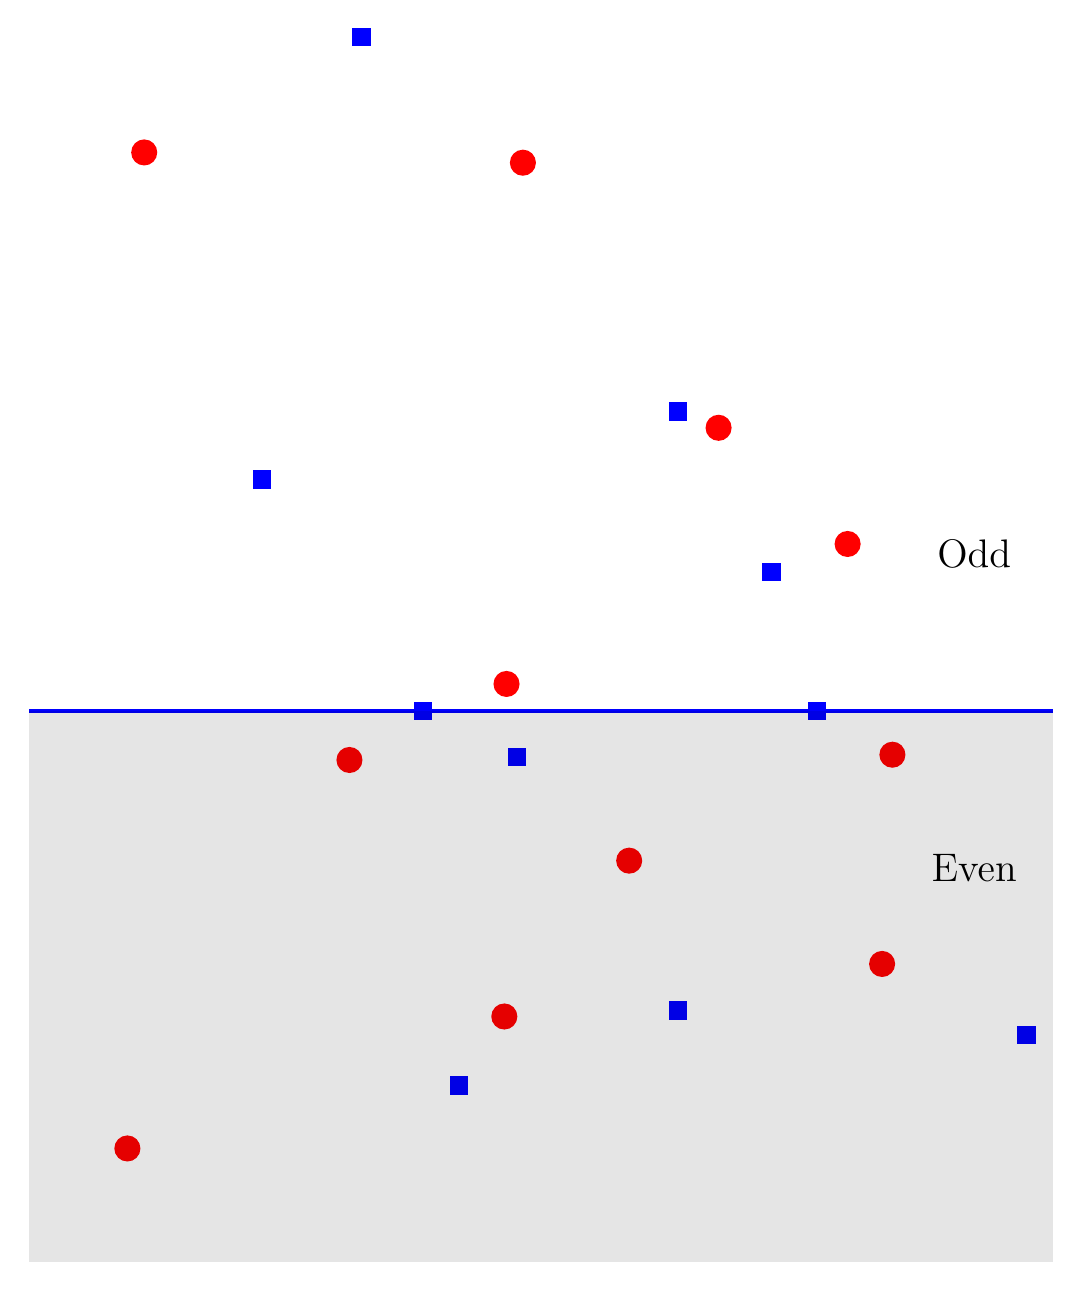
\begin{tikzpicture}
    \node[fill, \clrone] at (1*36:3) {};
    \node[fill, \clrone] at (2*36:4) {};
    \node[fill, \clrone] at (3*36:9) {};
    \node[fill, \clrone] at (4*36:5) {};
    \node[fill, \clrone] at (5*36:2) {};
    \node[fill, \clrone] at (6*36:1) {};
    \node[fill, \clrone] at (7*36:5) {};
    \node[fill, \clrone] at (8*36:4) {};
    \node[fill, \clrone] at (9*36:7) {};
    \node[fill, \clrone] at (10*36:3) {};

    \node[fill, circle, \clrtwo] at (1*32:4) {};
    \node[fill, circle, \clrtwo] at (2*32:4) {};
    \node[fill, circle, \clrtwo] at (3*32:7) {};
    \node[fill, circle, \clrtwo] at (4*32:9) {};
    \node[fill, circle, \clrtwo] at (5*32:1) {};
    \node[fill, circle, \clrtwo] at (6*32:3) {};
    \node[fill, circle, \clrtwo] at (7*32:8) {};
    \node[fill, circle, \clrtwo] at (8*32:4) {};
    \node[fill, circle, \clrtwo] at (9*32:2) {};
    \node[fill, circle, \clrtwo] at (10*32:5) {};
    \node[fill, circle, \clrtwo] at (11*32:4) {};

    \draw[blue, very thick] (-7,0) -- (6,0);
    \fill[opacity = 0.1] (-7,0) -- (-7,-7) -- (6,-7) -- (6,0) -- cycle;

    \node at (5,-2) {\Large Even};
    \node at (5,2) {\Large Odd};
\end{tikzpicture}


\end{document}